
\begin{figure}[H]
\centering
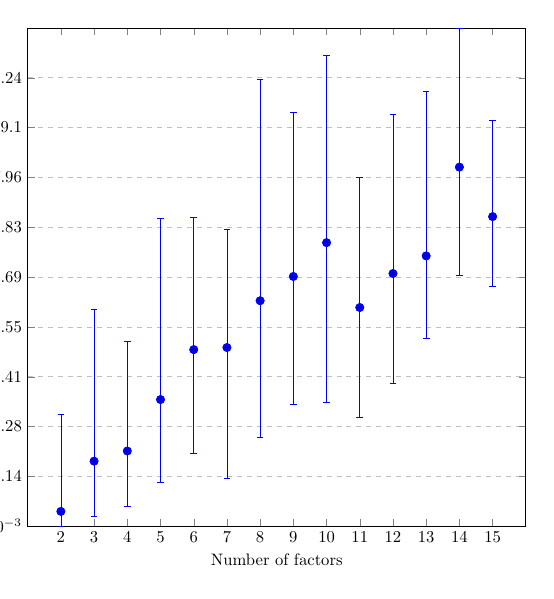
\begin{tikzpicture}[scale=0.6, trim axis left, trim axis right]
\begin{axis}[
    width=1\textwidth,
    height=1\textwidth,
    xlabel={Number of factors},
    ylabel={Time taken (s)},
    xmin=1.0, xmax=16.0,
    ymin=0.002547, ymax=11.373914,
    xticklabels={2, 3, 4, 5, 6, 7, 8, 9, 10, 11, 12, 13, 14, 15},
    xtick={2, 3, 4, 5, 6, 7, 8, 9, 10, 11, 12, 13, 14, 15},
    ytick={0.002547, 1.1396837, 2.2768204, 3.4139571, 4.5510938, 5.6882305, 6.8253672, 7.9625039, 9.0996406, 10.2367773},
    ymajorgrids=true,
    grid style=dashed,
]

\addplot+[
    blue,
    very thick,
    forget plot,
    only marks
    ]
    plot[
    very thick,
    error bars/.cd,
    y dir=plus,
    y explicit
    ]
    table[x=x,y=y,y error expr=\thisrow{y-max}] {
    x    y    y-max
    11	4.9933398	2.9658762
10	6.4743149	4.2694301
13	6.1712276	3.7602714
12	5.7694033	3.6381847
15	7.06889985714	2.20147214286
14	8.1986748	3.1752392
3	1.48588533333	3.45965266667
2	0.33928335	2.20725765
5	2.89246	4.145351
4	1.7181885	2.4993145
7	4.0801527	2.7018063
6	4.032296	3.030762
9	5.7020292	3.7549328
8	5.1483753	5.0619417

    };

\addplot+[
    blue,
    very thick,
    forget plot,
    only marks
    ]
    plot[
    very thick,
    error bars/.cd,
    y dir=plus,
    y explicit
    ]
    table[x=x,y=y,y error expr=\thisrow{y-min}] {
    x    y    y-min
    11	4.9933398	-2.5045318
10	6.4743149	-3.6536669
13	6.1712276	-1.8817726
12	5.7694033	-2.5004493
15	7.06889985714	-1.58310785714
14	8.1986748	-2.4808978
3	1.48588533333	-1.25647633333
2	0.33928335	-0.33673635
5	2.89246	-1.883798
4	1.7181885	-1.2688655
7	4.0801527	-2.9779397
6	4.032296	-2.366884
9	5.7020292	-2.9075462
8	5.1483753	-3.1277133

    };

\end{axis}
\end{tikzpicture}
\vspace{-0.3cm}
\caption{Large primes, stop after one iteration}\label{fig:LenstrasEllipticCurveFactorizationlargeprimes(maximumIterations:1)factors}
\end{figure}